\chapter{Concrete candidates for public key
crypto}\label{11-Concrete-candidates-fo}

In the previous lecture we talked about \emph{public key cryptography}
and saw the Diffie Hellman system and the DSA signature scheme. In this
lecture, we will see the RSA trapdoor function and how to use it for
both encryptions and signatures.

\section{Some number theory.}\label{11-Some-number-theory}

(See \href{http://www.shoup.net/ntb/}{Shoup's excellent and freely
available book} for extensive coverage of these and many other topics.)

For every number \(m\), we define \(\Z_m\) to be the set
\(\{0,\ldots,m-1\}\) with the addition and multiplication operations
modulo \(m\). When two elements are in \(\Z_n\) then we will always
assume that all operations are done modulo \(m\) unless stated
otherwise. We let \(\Z^*_m = \{ a\in \Z_m : gcd(a,m)=1 \}\). Note that
\(m\) is prime if and only if \(|\Z^*_m|=m-1\). For every
\(a \in \Z^*_m\) we can find using the extended gcd algorithm an element
\(b\) (typically denoted as \(a^{-1}\)) such that \(ab=1\) (can you see
why?). The set \(\Z^*_m\) is an abelian group with the multiplication
operation, and hence by the observations of the previous lecture,
\(a^{|\Z^*_m|}=1\) for every \(a\in \Z^*_m\). In the case that \(m\) is
prime, this result is known as ``Fermat's Little Theorem'' and is
typically stated as \(a^{p-1}=1 \pmod{p}\) for every \(a\neq 0\).

\hypertarget{smallvsbigrem}{}
\begin{remark}[Note on $n$ bits vs a number $n$] \label[remark]{smallvsbigrem}

One aspect that is often confusing in number-theoretic based
cryptography, is that one needs to always keep track whether we are
talking about ``big'' numbers or ``small'' numbers. In many cases in
crypto, we use \(n\) to talk about our key size or security parameter,
in which case we think of \(n\) as a ``small'' number of size
\(100-1000\) or so. However, when we work with \(\Z^*_m\) we often think
of \(m\) as a ``big'' number having about \(100-1000\) \emph{digits};
that is \(m\) would be roughly \(2^{100}\) to \(2^{1000}\) or so. I will
try to reserve the notation \(n\) for ``small'' numbers but may
sometimes forget to do so, and other descriptions of RSA etc.. often use
\(n\) for ``big'' numbers. It is important that whenever you see a
number \(x\), you make sure you have a sense whether it is a ``small''
number (in which case \(poly(x)\) time is considered efficient) or
whether it is a ``large'' number (in which case only \(poly(log(x))\)
time would be considered efficient).

\end{remark}

\hypertarget{numbermvsmessage}{}
\begin{remark}[The number $m$ vs the message $m$] \label[remark]{numbermvsmessage}

In much of this course we use \(m\) to denote a string which is our
plaintext message to be encrypted or authenticated. In the context of
integer factoring, it is convenient to use \(m=pq\) as the composite
number that is to be factored. To keep things interesting (or more
honestly, because I keep running out of letters) in this lecture we will
have both usages of \(m\) (though hopefully not in the same theorem or
definition!). When we talk about factoring, RSA, and Rabin, then we will
use \(m\) as the composite number, while in the context of the abstract
trapdoor-permutation based encryption and signatures we will use \(m\)
for the message. When you see an instance of \(m\), make sure you
understand what is its usage.

\end{remark}

\subsection{Primaliy testing}\label{11-Primaliy-testing}

One procedure we often need is to find a prime of \(n\) bits. The
typical way people do it is by choosing a random \(n\)-bit number \(p\),
and testing whether it is prime. We showed in the previous lecture that
a random \(n\) bit number is prime with probability at least
\(\Omega(1/n^2)\) (in fact the probability is
\(\tfrac{1\pm o(1)}{\ln n}\) by the \href{https://goo.gl/ChrXJY}{Prime
Number Theorem}). We now discuss how we can test for primality.

\hypertarget{primalitytesting}{}
\begin{theorem}[Primality Testing] \label[theorem]{primalitytesting}

There is an \(poly(n)\)-time algorithm to test whether a given \(n\)-bit
number is prime or composite.

\end{theorem}

\cref{primalitytesting} was first shown in 1970's by Solovay, Strassen,
Miller and Rabin via a \emph{probabilistic} algorithm (that can make a
mistake with probability exponentially small in the number of coins it
uses), and in a 2002 breakthrough Agrawal, Kayal, and Saxena gave a
\emph{deterministic} polynomial time algorithm for the same problem.

\hypertarget{pseudoprimelem}{}
\begin{lemma} \label[lemma]{pseudoprimelem}

There is a probabilistic polynomial time algorithm \(A\) that on input a
number \(m\), if \(m\) is prime \(A\) outputs \texttt{YES} with
probability \(1\) and if \(A\) is not even a ``pseudoprime'' it outputs
\texttt{NO} with probability at least \(1/2\). (The definition of
``pseudo-prime'' will be clarified in the proof below.)

\end{lemma}

\begin{proof} \label[proof]{11-The-algorithm-is-very-}

The algorithm is very simple and is based on Fermat's Little Theorem: on
input \(m\), pick a random \(a\in \{2,\ldots,m-1\}\), and if
\(gcd(a,m)\neq 1\) or \(a^{m-1} \neq 1 \pmod{m}\) return \texttt{NO} and
otherwise return \texttt{YES}.

By Fermat's little theorem, the algorithm will always return
\texttt{YES} on a prime \(m\). We define a ``pseudoprime'' to be a
non-prime number \(m\) such that \(a^{m-1}=1 \pmod{m}\) for all \(a\)
such that \(gcd(a,m)=1\).\\
If \(n\) is \emph{not} a pseudoprime then the set
\(S = \{ a\in\Z^*_m : a^{m-1}=1 \}\) is a strict subset of \(\Z^*_m\).
But it is easy to see that \(S\) is a \emph{group} and hence \(|S|\)
must divide \(|Z^*_n|\) and hence in particular it must be the case that
\(|S| < |\Z^*_n|/2\) and so with probability at least \(1/2\) the
algorithm will output \texttt{NO}.

\end{proof}

\cref{pseudoprimelem} its own might not seem very meaningful since it's
not clear how many pseudoprimes are there. However, it turns out these
pseudoprimes, also known as ``Carmichael numbers'', are much less
prevalent than the primes, specifically, there are about
\(N/2^{-\Theta(\log N/\log\log N)}\) pseudoprimes between \(1\) and
\(N\). If we choose a random number \(m \in [2^n]\) and output it if and
only if the algorithm of \cref{pseudoprimelem} algorithm outputs
\texttt{YES} (otherwise resampling), then the probability we make a
mistake and output a pseudoprime is equal to the ratio of the set of
pseudoprimes in \([2^n]\) to the set of primes in \([2^n]\). Since there
are \(\Omega(2^n/n)\) primes in \([2^n]\), this ratio is
\(\tfrac{n}{2^{-\Omega(n/\log n)}}\) which is a negligible quantity.
Moreover, as mentioned above, there are better algorithms that succeed
for \emph{all} numbers.

In contrast to \emph{testing} if a number is prime or composite, there
is no known efficient algorithm to actually \emph{find} the
factorization of a composite number. The best known algorithms run in
time roughly \(2^{\tilde{O}(n^{1/3})}\) where \(n\) is the number of
bits.

\subsection{Fields}\label{11-Fields}

If \(p\) is a prime then \(\Z_p\) is a \emph{field} which means it is
closed under addition and multiplication and has \(0\) and \(1\)
elements. One property of a field is the following:

\hypertarget{bezout}{}
\begin{theorem}[Fundamental Theorem of Algebra, mod $p$ version] \label[theorem]{bezout}

If \(f\) is a nonzero polynomial of degree \(d\) over \(\Z_p\) then
there are at most \(d\) distinct inputs \(x\) such that \(f(x)=0\).

\end{theorem}

(If you're curious why, you can see that the task of, given
\(x_1,\ldots,x_{d+1}\) finding the coefficients for a polynomial
vanishing on the \(x_i\)'s amounts to solving a linear system in \(d+1\)
variables with \(d+1\) equations that are independent due to the
non-singularity of the Vandermonde matrix.)

In particular every \(x \in \Z_p\) has at most two \emph{square roots}
(numbers \(s\) such that \(s^2 = x \mod p\)). In fact, just like over
the reals, every \(x\in\Z_p\) either has no square roots or exactly two
square roots of the form \(\pm s\).

We can efficiently find square roots modulo a prime. In fact, the
following result is known:

\hypertarget{rootfindingthm}{}
\begin{theorem}[Finding roots] \label[theorem]{rootfindingthm}

There is a probabilistic \(poly(\log p,d)\) time algorithm to find the
roots of a degree \(d\) polynomial over \(\Z_p\).

\end{theorem}

This is a special case of the problem of factoring polynomials over
finite fields, shown in 1967 by Berlekamp and on which much other work
has been done; see Chapter 20 in
\href{http://www.shoup.net/ntb/}{Shoup}).

\subsection{Chinese remainder theorem}\label{11-Chinese-remainder-theo}

Suppose that \(m=pq\) is a product of two primes. In this case \(Z^*_m\)
does not contain \emph{all} the numbers from \(1\) to \(m-1\). Indeed,
all the numbers of the form \(p,2p,3p,\ldots,(q-1)p\) and
\(q,2q,\ldots,(p-1)q\) will have non-trivial g.c.d. with \(m\). There
are exactly \(q-1 + p-1\) such numbers (because \(p\) and \(q\) are
prime all the numbers of the forms above are distinct). Hence
\(|Z^*_m| = m-1 - (p-1) - (q-1) = pq - p - q +1 = (p-1)(q-1)\).

Note that \(|Z^*_m|=|\Z^*_p|\cdot |\Z^*_q|\). It turns out this is no
accident:

\hypertarget{CRTthm}{}
\begin{theorem}[Chinese Remainder Theorem (CRT)] \label[theorem]{CRTthm}

If \(m=pq\) then there is an isomorphism
\(\varphi:\Z^*_m \rightarrow \Z^*_p \times \Z^*_q\). That is,
\(\varphi\) is one to one and onto and maps \(x\in\Z^*_m\) into a pair
\((\varphi_1(x),\varphi_2(x)) \in \Z^*_p \times \Z^*_q\) such that for
every \(x,y \in \Z^*_m\):\\
* \(\varphi_1(x+y) = \varphi_1(x)+\varphi_1(y) \pmod{p}\)\\
* \(\varphi_2(x+y) = \varphi_2(x)+\varphi_2(y) \pmod{q}\)\\
* \(\varphi_1(x\cdot y) = \varphi_1(x)\cdot \varphi_1(y) \pmod{p}\)\\
* \(\varphi_2(x\cdot y) = \varphi_2(x)\cdot \varphi_2(y) \pmod{q}\)

\end{theorem}

\begin{proof} \label[proof]{11-varphi-simply-maps-xin}

\(\varphi\) simply maps \(x\in \Z^*_m\) to the pair
\((x \mod p, x \mod q)\). Verifying that it satisfies all desired
properties is a good exercise. QED

\end{proof}

In particular, for every polynomial \(f()\) and \(x\in \Z^*_m\),
\(f(x)=0 \pmod{m}\) iff \(f(x)=0 \pmod{p}\) and \(f(x)=0 \pmod{q}\).
Therefore finding the roots of a polynomial \(f()\) modulo a composite
\(m\) is easy \emph{if you know \(m\)'s factorization}. However, if you
don't know the factorization then this is hard. In particular,
extracting square roots is as hard as finding out the factors:

\hypertarget{squarerootfactthm}{}
\begin{theorem}[Square root extraction implies factoring] \label[theorem]{squarerootfactthm}

Suppose and there is an efficient algorithm \(A\) such that for every
\(m\in \N\) and \(a\in \Z^*_m\), \(A(m,a^2 \pmod {m})=b\) such that
\(a^2 = b^2 \pmod{m}\). Then, there is an efficient algorithm to recover
\(p,q\) from \(m\).

\end{theorem}

\begin{proof} \label[proof]{11-Suppose-that-there-is-}

Suppose that there is such an algorithm \(A\). Using the CRT we can
define \(f:\Z^*_p\times\Z^*_q \rightarrow \Z^*_p\times \Z^*_q\) as
\(f(x,y)=\varphi(A(\varphi^{-1}(x^2,y^2)))\) for all \(x\in \Z^*_p\) and
\(y\in\Z^*_q\). Now, for any \(x,y\) let \((x',y')=f(x,y)\). Since
\(x^2 = x'^2 \pmod{p}\) and \(y^2 = y'^2 \pmod{q}\) we know that
\(x' \in \{\pm x \}\) and \(y' \in \{ \pm y \}\). Since flipping signs
doesn't change the value of \((x',y')=f(x,y)\), by flipping one or both
of the signs of \(x\) or \(y\) we can ensure that \(x'=x\) and
\(y'=-y\). Hence \((x,y)-(x',y')=(0,2y)\). In other words, if
\(c = \varphi^{-1}(x-x',y-y')\) then \(c= 0 \pmod{p}\) but
\(c \neq 0 \pmod{q}\) which in particular means that the greatest common
divisor of \(c\) and \(m\) is \(q\). So, by taking
\(gcd(A(\varphi^{-1}(x,y)),m)\) we will find \(q\), from which we can
find \(p=m/q\).

This almost works, but there is a question of how can we find
\(\varphi^{-1}(x,y)\), given that we don't know \(p\) and \(q\)? The
crucial observation is that we don't need to. We can simply pick a value
\(a\) at random in \(\{1,\ldots,m\}\). With very high probability
(namely \((p-1+q-1)/pq\)) \(a\) will be in \(\Z^*_m\), and so we can
imagine this process as equivalent to the process of taking a random
\(x\in\Z^*_p\), a random \(y\in \Z^*_q\) and then flipping the signs of
\(x\) and \(y\) randomly and taking \(a=\varphi(x,y)\). By the arguments
above with probability at least \(1/4\), it will hold that
\(gcd(a-A(a^2),m)\) will equal \(q\).

\end{proof}

Note that this argument generalizes to work even if the algorithm \(A\)
is an \emph{average case} algorithm that only succeeds in finding a
square root for a significant fraction of the inputs. This observation
is crucial for cryptographic applications.

\subsection{The RSA and Rabin
functions}\label{11-The-RSA-and-Rabin-func}

We are now ready to describe the RSA and Rabin trapdoor functions:

\hypertarget{RSAfuncdef}{}
\begin{definition}[RSA function] \label[definition]{RSAfuncdef}

Given a number \(m=pq\) and \(e\) such that \(gcd((p-1)(q-1),e)=1\), the
\emph{RSA function} w.r.t \(m\) and \(e\) is the map
\(f_{m,e}:\Z^*_m\rightarrow\Z^*_m\) such that
\(\ensuremath{\mathit{RSA}}_{m,e}(x) = x^e \pmod{m}\).

\end{definition}

\hypertarget{Rabinfuncdef}{}
\begin{definition}[Rabin function] \label[definition]{Rabinfuncdef}

Given a number \(m=pq\), the \emph{Rabin function} w.r.t. \(m\), is the
map \(Rabin_m:\Z^*_m\rightarrow \Z^*_m\) such that
\(Rabin_m(x)=x^2 \pmod{m}\).

\end{definition}

Note that both maps can be computed in polynomial time. Using the
Chinese Remainder Theorem and \cref{rootfindingthm}, we know that both
functions can be \emph{inverted} efficiently if we know the
factorization.\footnote{Using \cref{rootfindingthm} to invert the
  function requires \(e\) to be not too large. However, as we will see
  below it turns out that using the factorization we can invert the RSA
  function for every \(e\). Also, in practice people often use a small
  value for \(e\) (sometimes as small as \(e=3\)) for reasons of
  efficiency.}\\
However \cref{rootfindingthm} is a much too big of a Hammer to invert
the RSA and Rabin functions, and there are direct and simple inversion
algorithms (see homework exercises). By \cref{squarerootfactthm},
inverting the Rabin function amounts to factoring \(m\). No such result
is known for the RSA function, but there is no better algorithm known to
attack it than proceeding via factorization of \(m\). The RSA function
has the advantage that it is a \emph{permutation} over \(\Z^*_m\):

\hypertarget{RSAonetoonelem}{}
\begin{lemma} \label[lemma]{RSAonetoonelem}

\(\ensuremath{\mathit{RSA}}_{m,e}\) is one to one over \(\Z^*_m\).

\end{lemma}

\begin{proof} \label[proof]{11-Suppose-that-ensuremat}

Suppose that
\(\ensuremath{\mathit{RSA}}_{m,e}(a)=\ensuremath{\mathit{RSA}}_{m,e}(a')\).
By the CRT, it means that there is
\((x,y) \neq (x',y') \in \Z^*_p \times \Z^*_q\) such that
\(x^e = x'^e \pmod{p}\) and \(y^e = y'^e \pmod{q}\). But if that's the
case we get that \((xx'^{-1})^e = 1 \pmod{p}\) and
\((yy'^{-1})^e = 1 \pmod{q}\). But this means that \(e\) has to be a
multiple of the \emph{order} of \(xx'^{-1}\) and \(yy'^{-1}\) (at least
one of which is \emph{not} \(1\) and hence has order \(>1\)). But since
the order always divides the group size, this implies that \(e\) has to
have non-trivial gcd with either \(|Z^*_p|\) or \(|\Z^*_q|\) and hence
with \((p-1)(q-1)\).

\end{proof}

\hypertarget{plainrsarem}{}
\begin{remark}[Plain/Textbook RSA] \label[remark]{plainrsarem}

The RSA trapdoor function is known also as ``plain'' or ``textbook'' RSA
encryption. This is because initially Diffie and Hellman (and following
them, RSA) thought of an encryption scheme as a deterministic procedure
and so considered simply encrypting a message \(x\) by applying
\(\ensuremath{\mathit{ESA}}_{m,e}(x)\). Today however we know that it is
insecure to use a trapdoor function directly as an encryption scheme
without adding some randomization.

\end{remark}

\subsection{Abstraction: trapdoor
permutations}\label{11-Abstraction-trapdoor-p}

We can abstract away the particular construction of the RSA and Rabin
functions to talk about a general \emph{trapdoor permutation family}. We
make the following definition

\hypertarget{TDPdef}{}
\begin{definition}[Trapdoor permutation] \label[definition]{TDPdef}

A \emph{trapdoor permutation family (TDP)} is a family of functions
\(\{ p_k \}\) such that for every \(k\in\{0,1\}^n\), the function
\(p_k\) is a permutation on \(\{0,1\}^n\) and:\\
* There is a \emph{key generation algorithm} \(G\) such that on input
\(1^n\) it outputs a pair \((k,\tau)\) such that the maps
\(k,x \mapsto p_k(x)\) and \(\tau,y \mapsto p_k^{-1}(y)\) are
efficiently computable.

\begin{itemize}
\tightlist
\item
  For every efficient adversary \(A\),
  \(\Pr_{(k,\tau) \leftarrow_R G(1^n), y\in\{0,1\}^n}[ A(k,y)=p_k^{-1}(y) ] < negl(n)\).\\
\end{itemize}

\end{definition}

\hfill\break

\hfill\break

\hypertarget{permutationsovergroups}{}
\begin{remark}[Domain of permutations] \label[remark]{permutationsovergroups}

The RSA function is not a permutation over the set of strings but rather
over \(\Z^*_m\) for some \(m=pq\). However, if we find primes \(p,q\) in
the interval \([2^{n/2}(1-negl(n)),2^{n/2}]\), then \(m\) will be in the
interval \([2^n(1-negl(n)),2^n]\) and hence \(\Z^*_m\) (which has size
\(pq - p - q +1 = 2^n(1-negl(n))\)) can be thought of as essentially
identical to \(\{0,1\}^n\), since we will always pick elements from
\(\{0,1\}^n\) at random and hence they will be in \(\Z^*_m\) with
probability \(1-negl(n)\). It is widely believed that for every
sufficiently large \(n\) there is a prime in the interval
\([2^n-poly(n),2^n]\) (this follows from the \emph{Extended Reimann
Hypothesis}) and Baker, Harman and Pintz \emph{proved} that there is a
prime in the interval \([2^n-2^{0.6n},2^n]\).\footnote{Another, more
  minor issue is that the description of the key might not have the same
  length as \(\log m\); I defined them to be the same for simplicity of
  notation, and this can be ensured via some padding and concatenation
  tricks.}

\end{remark}

\subsection{Public key encryption from trapdoor
permutations}\label{11-Public-key-encryption-}

Here is how we can get a public key encryption from a trapdoor
permutation scheme \(\{ p_k \}\).

\begin{quote}
\textbf{TDP-based public key encryption (TDPENC):}

\begin{itemize}
\item
  \emph{Key generation:} Run the key generation algorithm of the TDP to
  get \((k,\tau)\). \(k\) is the \emph{public encryption key} and
  \(\tau\) is the \emph{secret decryption key}.
\item
  \emph{Encryption:} To encrypt a message \(m\) with key
  \(k\in\{0,1\}^n\), choose \(x\in\{0,1\}^n\) and output
  \((p_k(x),H(x)\oplus m)\) where \(H:\{0,1\}^n\rightarrow\{0,1\}^\ell\)
  is a hash function we model as a random oracle.
\item
  \emph{Decryption:} To decrypt the ciphertext \((y,z)\) with key
  \(\tau\), output \(m=H(p_k^{-1}(y))\oplus z\).
\end{itemize}
\end{quote}

\begin{pause} \label[pause]{11-Please-verify-that-you}

Please verify that you understand why TDPENC is a \emph{valid}
encryption scheme, in the sense that decryption of an encryption of
\(m\) yields \(m\).

\end{pause}

\hypertarget{TDPpkcthm}{}
\begin{theorem}[Public key encryption from trapdoor permutations] \label[theorem]{TDPpkcthm}

If \(\{ p_k \}\) is a secure TDP and \(H\) is a random oracle then
TDPENC is a CPA secure public key encryption scheme.

\end{theorem}

\begin{proof} \label[proof]{11-Suppose-towards-the-sa}

Suppose, towards the sake of contradiction, that there is a
polynomial-size adversary \(A\) that succeeds in the CPA game of TDPENC
(with access to a random oracle \(H\)) with non-negligible advantage
\(\epsilon\) over half. We will use \(A\) to design an algorithm \(I\)
that inverts the trapdoor permutation.

Recall that the CPA game works as follows:

\begin{itemize}
\item
  The adversary \(A\) gets as input a key \(k \in \{0,1\}^n\).
\item
  The algorithm \(A\) makes some polynomial amount of computation and
  \(T_1=poly(n)\) queries to the random oracle \(H\) and produces a pair
  of messages \(m_0,m_1 \in \{0,1\}^\ell\).
\item
  The ``challenger'' chooses \(b^* \leftarrow_R \{0,1\}\), chooses
  \(x^* \leftarrow_R \{0,1\}^n\) and computes the ciphertext
  \((y^*=p_k(x^*),z^* = H(x^*) \oplus m_{b^*})\) which is an encryption
  of \(m_{b^*}\).
\item
  The adversary \(A\) gets \((y^*,z^*)\) as input, makes some additional
  polynomial amount of computation and \(T_2=poly(n)\) queries to \(H\),
  and then outputs \(b\).
\item
  The adversary \emph{wins} if \(b=b^*\).
\end{itemize}

We make the following claim:

\textbf{CLAIM:} With probability at least \(\epsilon\), the adversary
\(A\) will make the query \(x^*\) to the random oracle.

\textbf{PROOF:} Suppose otherwise. We will prove the claim using the
``forgetful gnome'' technique as used in the Boneh Shoup book. By the
``lazy evaluation'' paradigm, we can imagine that queries to \(H\) are
answered by a ``faithful gnome'' that whenever presented with a new
query \(x\), chooses a uniform and independent value
\(w \leftarrow_R \{0,1\}^\ell\) as a response, and then records that
\(H(x)=w\) to use that as answers for future queries.

Now consider the experiment where in the challenge part we use a
``forgetful gnome'' that answers \(H(x^*)\) by a uniform and independent
string \(w^* \leftarrow_R \{0,1\}^\ell\) and \emph{does not} record the
answer for future queries. In the ``forgetful experiment'', the second
component of the ciphertext \(z^* = w^* \oplus m_{b^*}\) is distributed
uniformly in \(\{0,1\}^\ell\) and independently from all other random
choices, regardless of whether \(b^*=0\) or \(b^*=1\). Hence in this
``forgetful experiment'' the adversary gets no information about \(b^*\)
and its probability of winning is at most \(1/2\). But the forgetful
experiment is identical to the actual experiment if the value \(x^*\) is
only queried to \(H\) once. Apart from the query of \(x^*\) by the
challenger, all other queries to \(H\) are made by the adversary. Under
our assumption, the adversary makes the query \(x^*\) with probability
at most \(\epsilon\), and conditioned on this not happening the two
experiments are identical. Since the probability of winning in the
forgetful experiment is at most \(1/2\), the probability of winning in
the overall experiment is less than \(1/2+\epsilon\), thus yielding a
contradiction and establishing the claim. (These kind of analyses on
sample spaces can be confusing; See \cref{TDPENCgnomefig} for a
graphical illustration of this argument.)

Given the claim, we can now construct our inverter algorithm \(I\) as
follows:

\begin{itemize}
\item
  The input to \(I\) is the key \(k\) to the trapdoor permutation and
  \(y^* = p_k(x^*)\). The goal of \(I\) is to output \(x^*\).
\item
  The inverter simulates the adversary in a CPA attack, answering all
  its queries to the oracle \(H\) by random values if they are new or
  the previously supplied answers if they were asked before. Whenever
  the adversary makes a query \(x\) to \(H\), \(I\) checks if
  \(p_h(x)=y^*\) and if so halts and outputs \(x\).
\item
  When the time comes to produce the challenge, the inverter \(I\)
  chooses \(z^*\) at random and provides the adversary with
  \((y^*,z^*)\) where \(z^* = w^* \oplus m_{b^*}\).\footnote{It would
    have been equivalent to answer the adversary with a uniformly chosen
    \(z^*\) in \(\{0,1\}^\ell\), can you see why?}
\item
  The inverter continues the simulation again halting an outputting
  \(x\) if the adversary makes the query \(x\) such that \(p_k(x)=y^*\)
  to \(H\).
\end{itemize}

We claim that up to the point we halt, the experiment is identical to
the actual attack. Indeed, since \(p_k\) is a permutation, we know that
if the time came to produce the challenge and we have not halted, then
the query \(x^*\) has not been made yet to \(H\). Therefore we are free
to choose an independent random value \(w^*\) as the value \(H(x^*)\).
(Our inverter does not know what the value \(x^*\) is, but this does not
matter for this argument: can you see why?) Therefore, since by the
claim the adversary will make the query \(x^*\) to \(H\) with
probability at least \(\epsilon\), our inverter will succeed with the
same probability.

\end{proof}

\begin{marginfigure}
\centering
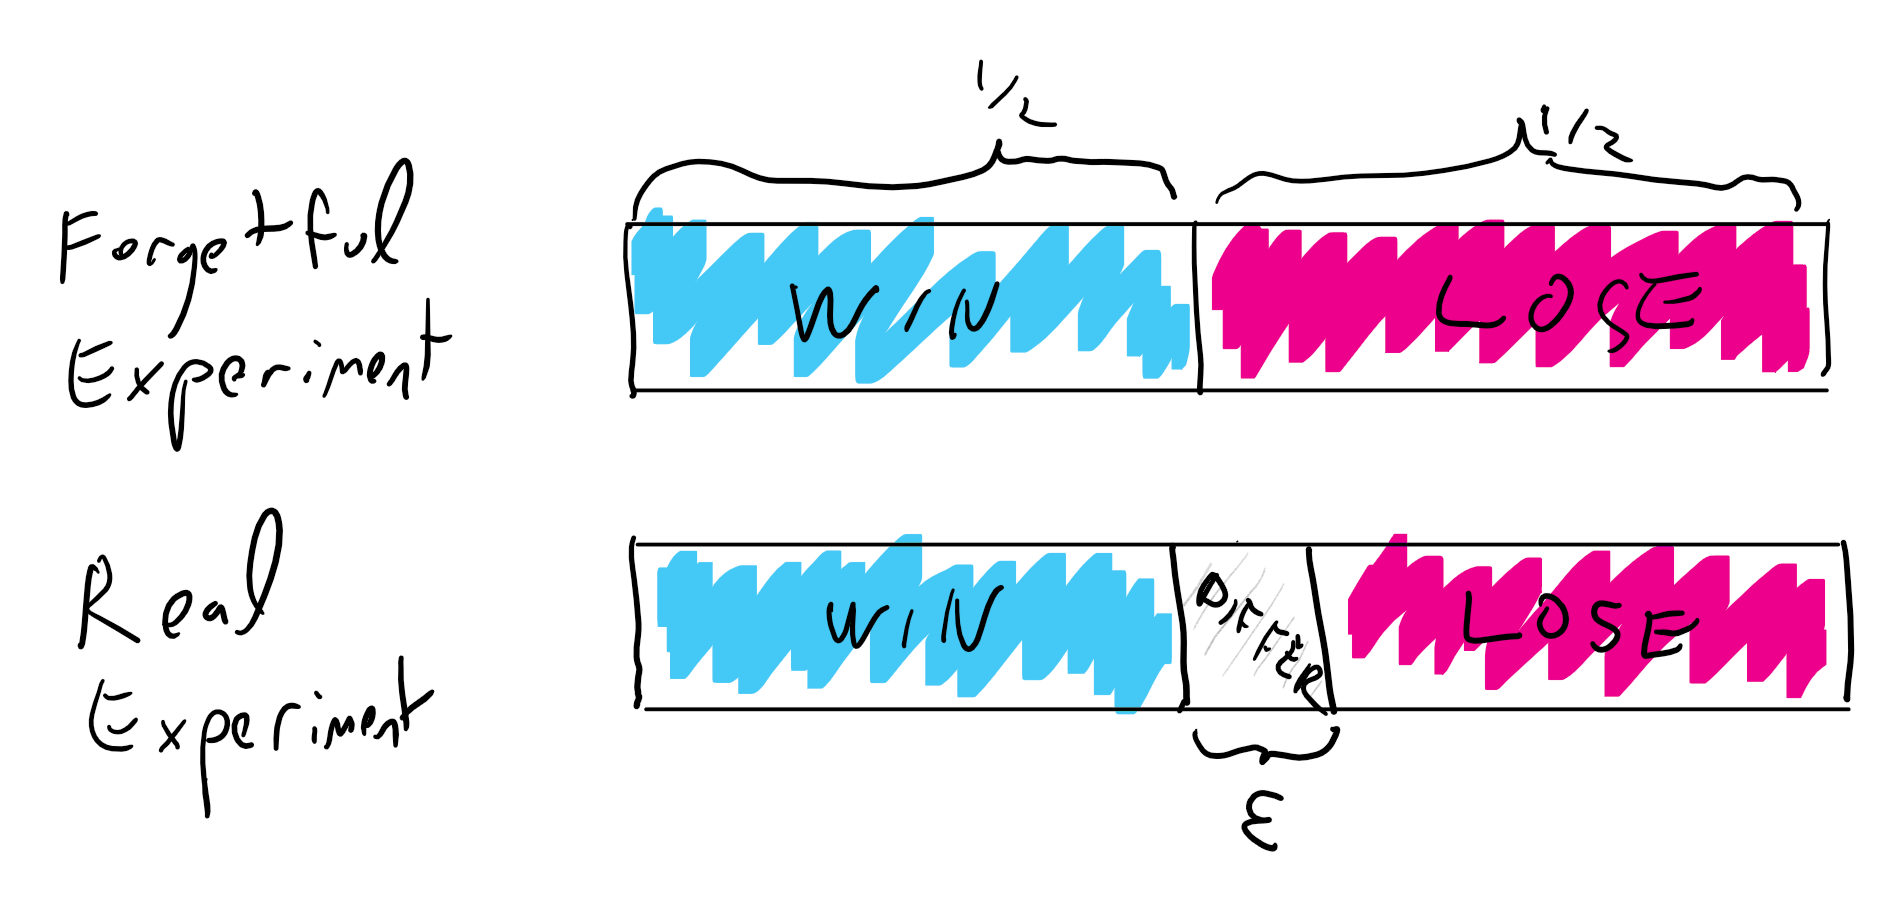
\includegraphics[width=\linewidth, height=1.5in, keepaspectratio]{../figure/gnomeTDPENC.png}
\caption{In the proof of security of TDPENC, we show that if the
assumption of the claim is violated, the ``forgetful experiment'' is
identical to the real experiment with probability larger \(1-\epsilon\).
In such a case, even if all that probability mass was on the points in
the sample space where the adversary in the forgetful experiment will
lose and the adversary of the real experiment will win, the probability
of winning in the latter experiment would still be less than
\(1/2+\epsilon\).}
\label{TDPENCgnomefig}
\end{marginfigure}

\begin{pause} \label[pause]{11-This-proof-of-crefTDPp}

This proof of \cref{TDPpkcthm} is not very long but it is somewhat
subtle. Please re-read it and make sure you understand it. I also
recommend you look at the version of the same proof in Boneh Shoup:
Theorem 11.2 in Section 11.4 (``Encryption based on a trapdoor function
scheme'').

\end{pause}

\hypertarget{noromtdpthm}{}
\begin{remark}[Security without random oracles] \label[remark]{noromtdpthm}

We do \emph{not} need to use a random oracle to get security in this
scheme, especially if \(\ell\) is sufficiently short. We can replace
\(H()\) with a hash function of specific properties known as a
\emph{hard core} construction; this was first shown by Goldreich and
Levin.

\end{remark}

\subsection{Digital signatures from trapdoor
permutations}\label{11-Digital-signatures-fro}

Here is how we can get digital signatures from trapdoor permutations
\(\{ p_k \}\). This is known as the ``full domain hash'' signatures.

\begin{quote}
\textbf{Full domain hash signatures (FDHSIG):}

\begin{itemize}
\item
  \emph{Key generation:} Run the key generation algorithm of the TDP to
  get \((k,\tau)\). \(k\) is the \emph{public verification key} and
  \(\tau\) is the \emph{secret signing key}.
\item
  \emph{Signing:} To sign a message \(m\) with key \(\tau\), we output
  \(p_{k}^{-1}(H(m))\) where \(H:\{0,1\}^*\rightarrow\{0,1\}^n\) is a
  hash function modeled as a random oracle.
\item
  \emph{Verification:} To verify a message-signature pair \((m,x)\) we
  check that \(p_k(x)=H(m)\).
\end{itemize}
\end{quote}

We now prove the security of full domain hash:

\hypertarget{FDHthm}{}
\begin{theorem}[Full domain hash security] \label[theorem]{FDHthm}

If \(\{ p_k \}\) is a secure TDP and \(H\) is a random oracle then
FDHSIG is chosen message attack secure digital signature scheme.

\end{theorem}

\begin{proof} \label[proof]{11-Suppose-towards-the-sa}

Suppose towards the sake of contradiction that there is a
polynomial-sized adversary \(A\) that succeeds in a chosen message
attack with non-negligible probability \(\epsilon>0\). We will construct
an inverter \(I\) for the trapdoor permutation collection that succeeds
with non-negligible probability as well.

Recall that in a chosen message attack the adversary makes \(T\) queries
\(m_1,\ldots,m_T\) to its signing box which are interspersed with \(T'\)
queries \(m'_1,\ldots,m'_{T'}\) to the random oracle \(H\). We can
assume without loss of generality (by modifying the adversary and at
most doubling the number of queries) that the adversary always queries
the message \(m_i\) to the random oracle \emph{before} it queries it to
the signing box, though it can also make additional queries to the
random oracle (and hence in particular \(T' \geq T\)). At the end of the
attack the adversary outputs with probability \(\epsilon\) a pair
\((x^*,m^*)\) such that \(m^*\) was not queried to the signing box and
\(p_k(x^*)=H(m^*)\).

Our inverter \(I\) works as follows:

\begin{itemize}
\item
  \textbf{Input:} \(k\) and \(y^*=p_k(y^*)\). Goal is to output \(x^*\).
\item
  \(I\) will guess at random \(t^*\) which is the step in which the
  adversary will query to \(H\) the message \(m^*\) that it is
  eventually going to forge in. With probability \(1/T'\) the guess will
  be correct.
\item
  \(I\) simulates the execution of \(A\). Except for step \(t^*\),
  whenever \(A\) makes a new query \(m\) to the random oracle, \(I\)
  will choose a random \(x\leftarrow \{0,1\}^n\), compute \(y=p_k(x)\)
  and designate \(H(m)=y\). In step \(t^*\), when the adversary makes
  the query \(m^*\), the inverter \(I\) will return \(H(m^*)=y^*\).
  \(I\) will record the values \((x,y)\) and so in particular will
  always know \(p_k^{-1}(H(m))\) for every \(H(m) \neq y^*\) that it
  returned as answer from its oracle on query \(m\).
\item
  When \(A\) makes the query \(m\) to the signature box, then since
  \(m\) was queried before to \(H\), if \(m \neq m^*\) then \(I\)
  returns \(x=p_k^{-1}(H(m))\) using its records. If \(m=m^*\) then
  \(I\) halts and outputs ``failure''.
\item
  At the end of the game, the adversary outputs \((m^*,x^*)\). If
  \(p_k(x^*)=y^*\) then \(I\) outputs \(x^*\).
\end{itemize}

We claim that, conditioned on the probability \(\geq \epsilon/T'\) event
that the adversary is successful and the final message \(m^*\) is the
one queried in step \(t^*\), we provide a perfect simulation of the
actual game. Indeed, while in an actual game, the value \(y=H(m)\) will
be chosen independently at random in \(\{0,1\}^n\), this is equivalent
to choosing \(x \leftarrow_R \{0,1\}^n\) and letting \(y=p_k(x)\). After
all, a permutation applied to the uniform distribution is uniform.

Therefore with probability at least \(\epsilon/T'\) the inverter \(I\)
will output \(x^*\) such that \(p_k(x^*)=y^*\) hence succeeding in the
inverter.

\end{proof}

\begin{pause} \label[pause]{11-Once-again-this-proof-}

Once again, this proof is somewhat subtle. I recommend you also read the
version of this proof in Section 13.4 of Boneh-Shoup.

\end{pause}

\hypertarget{hashandsignrem}{}
\begin{remark}[Hash and sign] \label[remark]{hashandsignrem}

There is another reason to use hash functions with signatures. By
combining a collision-resistant hash function
\(h:\{0,1\}^* \rightarrow \{0,1\}^\ell\) with a signature scheme
\((S,V)\) for \(\ell\)-length messages, we can obtain a signature for
arbitrary length messages by defining \(S'_s(m)=S_s(h(m))\) and
\(V'_v(m,\sigma)=V_v(h(m),\sigma)\).

\end{remark}

\section{Hardcore bits and security without random
oracles}\label{11-Hardcore-bits-and-secu}

The main problem with using trapdoor functions as the basis of public
key encryption is twofold: \textgreater{} * The fact that \(f\) is a
trapdoor function does not rule out the possibility of computing \(x\)
from \(f(x)\) when \(x\) is of some special form. Recall that the
security of a one-way function is given over a uniformly random input.
Usually messages to be sent are not drawn from a uniform distribution,
and it's possible that for some certain values of \(x\) it is easy to
invert \(f(x)\), and those values of \(x\) also happen to be commonly
sent messages. \textgreater{} * The fact that \(f\) is a trapdoor
function does not rule out the possiblity of easily computing some
partial information about \(x\) from \(f(x)\). Suppose we wished to play
poker over a channel of bits. If even the suit or color of a card can be
revealed from the encryption of that card, then it doesn't matter if the
entire encryption cannot be inverted; being able to compute even a
single bit of the plaintext makes the entire game invalid. The RSA and
Rabin functions have not been successfully reversed, but nobody has been
able to prove that they give \emph{semantic security}. \textgreater{}
The solution to these issues is to use a hardcore predicate of a one-way
function \(f\). We first define the security of a hardcore predicate,
then show how it can be used to construct semantically secure
encryption.

\hypertarget{HCPdef}{}
\begin{definition}[Hardcore predicate] \label[definition]{HCPdef}

Let \(f:\{0, 1\}^n \rightarrow \{0, 1\}^n\) be a one-way function (we
assume \(f\) is length preserving for simplicity), \(\ell(n)\) be a
length function, and \(h: \{0, 1\}^n \rightarrow \{0, 1\}^{\ell(n)}\) be
polynomial time computable. We say \(h\) is a \textbf{hardcore
predicate} of \(f\) if for every efficient adversary \(A\), every
polynomial \(p\), and all sufficiently large \(n\),
\begin{equation*}
\left| \Pr[A(f(X_n), b(X_n)) = 1] - \Pr[A(f(X_n), R_{\ell(n)}) = 1]\right| < \frac{1}{p(n)}
\end{equation*}
where \(X_n\) and \(R_{\ell(n)}\) are independently and uniformly
distributed over \(\{0, 1\}^n\) and \(\{0, 1\}^{\ell(n)}\),
respectively.

\end{definition}

That is, given an input \(x \leftarrow_R \{0, 1\}^n\) chosen uniformly
at random, no efficient adversary can distingusih between a random
string \(r\) and \(b(x)\) given \(f(x)\) with non negligible advantage.
This allows us to construct semantically secure public key encryption:

\begin{quote}
\textbf{Hardcore predicate-based public key encryption:}

\begin{itemize}
\item
  \emph{Key generation:} Run the standard key generation algorithm for
  the one-way function \(f\) to get \((e, d)\), where \(e\) is a public
  key used to compute the function \(f\) and \(d\) is a corresponding
  secret trapdoor key that makes it easy to invert \(f\).
\item
  \emph{Encryption:} To encrypt a message \(m\) of length \(n\) with
  public key \(e\), pick \(x \leftarrow_R \{0, 1\}^n\) uniformly at
  random and compute \((f_e(x), b(x) \oplus m)\).
\end{itemize}
\end{quote}

\begin{itemize}
\tightlist
\item
  \emph{Decryption:} To decrypt the ciphertext \((c, c')\) we first use
  the secret trapdoor key \(d\) to compute \(D_d(c) = D_d(f_e(x)) = x\),
  then compute \(b(x)\) and \(b(x) \oplus c' = m\)
\end{itemize}

\begin{pause} \label[pause]{11-Please-stop-to-verify-}

Please stop to verify that this is a valid public key encryption scheme.

\end{pause}

\begin{quote}
Note that in this construction of public key encryption, the input to
\(f\) is \(x\) drawn uniformly at random from \(\{0, 1\}^n\), so the
defininition of the one-wayness of \(f\) can be applied directly.
Furthermore, since \(b(x)\) is indistinguishable from a random string
\(r\) even given \(f(x)\), the output \(b(x) \oplus m\) is essentially a
one-time pad encryption of \(m\), where the key can only be retrieved by
someone who can invert \(f\). Proving the security formally is left as
an exercise.
\end{quote}

\begin{quote}
This is all fine and good, but how do we actually construct a hardcore
predicate? Blum and Micali were the first to construct a hardcore
predicate based on the discrete logarithm problem, but the first
construction for general one-way functions was given by Goldreich and
Levin. Their idea is that if \(f\) is one-way, then it's hard to guess
the exclusive or of a random subset of the input to \(f\) when given
\(f(x)\) and the subset itself.
\end{quote}

\hypertarget{HCBthm}{}
\begin{theorem}[A hardcore predicate for arbitrary one-way functions] \label[theorem]{HCBthm}

Let \(f\) be a one-way function, and let \(g\) be defined as
\(g(x, r) = (f(x), r)\), where \(|x| = |r|\). Let
\(b(x, r) = \oplus_{i \in [n]} x_ir_i\) be the inner product \(\mod 2\)
of \(x\) and \(r\). Then \(b\) is a hard core predicate of the function
\(g\).

\end{theorem}

\begin{quote}
The proof of this theorem follows the classic proof by reduction method,
where we assume the existence of an adversary that can predict
\(b(x, r)\) given \(g(x, r)\) with non negligible advantage and
construct an adversary that inverts \(f\) with non negligible
probability. Let \(A\) be a (possibly randomized) program and
\(\epsilon_A(n) > \tfrac{1}{p(n)}\) for some polynomial \(n\) such that
\end{quote}

\begin{equation*}
\Pr[A(g(X_n, R_n)) = b(X_n, R_n)] = \tfrac{1}{2} + \epsilon_A(n)
\end{equation*}

Where \(X_n\) and \(R_n\) are uniform and independent distributions over
\(\{0, 1\}^n\). We observe that \(b\) being insecure and having an
output of a single bit implies that such a program \(A\) exists. First,
we show that on at least \(\epsilon_A(n)\) fraction of the possible
inputs, program \(A\) has a \(\tfrac{\epsilon_A(n)}{2}\) advantage in
predicting the output of \(b\).

\hypertarget{EpsilonAdv}{}
\begin{lemma} \label[lemma]{EpsilonAdv}

There exists a set \(S \subseteq \{0, 1\}^n\) where
\(|S| > \epsilon_A(n) (2^n)\) such that for all \(x \in S\),

\end{lemma}

\begin{equation*}
s(x) = \Pr[A(g(x, R_n)) = b(x, R_n)] \geq \frac{1}{2} + \frac{\epsilon_A(n)}{2}
\end{equation*}

\begin{proof} \label[proof]{11-The-result-follows-fro}

The result follows from an averaging argument. Let
\(k = \frac{|S|}{2^n}\),
\(\displaystyle \alpha = \frac{1}{k} \sum_{x \in S} s(x)\) and
\(\displaystyle \beta = \frac{1}{1 - k} \sum_{x \notin S} s(x)\) be the
averages of \(s(x)\) over values in and not in \(S\), respectively, so
\(k \alpha + (1 - k) \beta = \frac{1}{2} + \epsilon\). For notational
convenience we set \(\epsilon = \epsilon_A(n)\). By definition
\(\mathbb{E}[s(X_n)] = \frac{1}{2} + \epsilon\), so the fact that
\(\alpha \leq 1\) and \(\beta < \frac{1}{2} + \frac{\epsilon}{2}\) gives
\(k + (1 - k) \left( \frac{1}{2} + \frac{\epsilon}{2} \right) > \frac{1}{2} + \epsilon\),
and solving finds that \(k > \epsilon\).

\end{proof}

\begin{quote}
Now we observe that for any \(r \in \{0, 1\}^n\), we have
\end{quote}

\begin{equation*}
x_i = b(x, r) \oplus b(x, r \oplus e_i)
\end{equation*}

where \(e_i\) is the vector with all \(0\)s except a \(1\) in the
\(i\)th location. This observation follows from the definition of \(b\),
and it motivates the main idea of the reduction: Guess \(b(x, r)\) and
use \(A\) to compute \(b(x, r \oplus e_i)\), then put it together to
find \(x_i\) for all \(i\). The reason guessing works will become clear
later, but intuitively the reason we cannot simply use \(A\) to compute
both \(b(x, r)\) and \(b(x, r \oplus e_i)\) is that the probability
\(A\) guesses both correctly is only (standard union) bounded below by
\(1 - 2 \left( \tfrac{1}{2} - \epsilon_A(n)\right) = 2\epsilon_A(n)\).
However, if we can guess \(b(x, r)\) correctly, then we only need to
invoke \(A\) one time to get a better than half probability of correctly
determining \(x_i\). It is then a simple matter of taking a majority
vote over several such \(r\) to determine each \(x_i\).

\begin{quote}
Now the natural question is how can we possibly guess (and here we
literally mean randomly guess) each value of \(b(x, r)\)? The key is
that the values of \(r\) only need to be \emph{pairwise} independent,
since down the line we plan to use Chebyshev's inequality on the
accuracy of our guesses\footnote{This has to do with the fact that
  Chebyshev's inequality is based on the variances of random variables.
  If we had to use the Chernoff bound we would be in trouble, since that
  requires full independence. For more on these and other concentration
  bounds, we recommend referring to the text Probability and Computing,
  by Eli Upfal.}. This means that while we need \(poly(n)\) many values
of \(r\), we can get away with guessing \(\log (n)\) values of
\(b(x, r)\) and combining them with some trickery to get more while
preserving pairwise independence. Since \(2^{-\log n} = \tfrac{1}{n}\),
with non negligible probability we can correctly guess all of our
\(b(x, r)\) for polynomially many \(r\). We then use \(A\) to compute
\(b(x, r \oplus e_i)\) for all \(r\) and \(i\), and since \(A\) has a
non negligible advantage by majority vote we can retrieve each value of
\(x_i\) to invert \(f\), thus contradicting the one-wayness of \(f\).
\end{quote}

\begin{pause} \label[pause]{11-It-is-important-that-y}

It is important that you understand why we cannot rely on invoking \(A\)
twice, on both \(b(x, r)\) and \(b(x, r \oplus e_i)\). It is also
important that you understand why, with non neligible probability, we
can correctly guess \(b(x, r_1), \dots b(x, r_\ell)\) for
\(r_1, \dots r_\ell\) chosen independently and uniformly at random and
\(\ell = O(\log n)\). At the moment, it is not important what trickery
is used to combine our guesses, but it will reduce confusion down the
line if you understand why we can get away with pairwise independence in
our inputs instead of complete mutual independence.

\end{pause}

Before moving on to the formal proof of our theorem, please stop to
convince yourself that, given that some trickery exists, this strategy
works for inverting \(f\).

\begin{proof}[Proof of \cref{HCBthm}] \label[proof]{temp}

\end{proof}

We use the assumed existence of \(A\) to construct \(B\), a program that
inverts \(f\) (which we assume is length preserving for notational
convenience). Pick \(n = |x|\) and
\(l = \lceil \log(2n \cdot p(n)^2 + 1) \rceil\), where
\(\epsilon_A(n) > \tfrac{1}{p(n)}\). Next, choose
\(s^1, \dots s^l \in \{0, 1\}^n\) and
\(\sigma^1, \dots \sigma^l \in \{0, 1\}\) all independently and
uniformly at random. Here we set \(\sigma^i\) to be the guess for the
value of \(b(x, s^i)\). For each non-empty subset \(J\) of
\(\{1, 2, \dots l\}\) let \(r^J = \oplus_{j \in J} s^j\). We can observe
that

\begin{equation*}
b(x, r^J) = b(x, \oplus_{j \in J} s^j) = \oplus_{j \in J} b(x, s^j)
\end{equation*}

by the properties of addition modulo 2, so we can say
\(\rho^J = \oplus_{j \in J} \sigma^j\) is the correct guess for
\(b(x, r^J)\) as long as each of \(\sigma^j\) for \(j \in J\) are
correct. We can easily verify that the values \(r^J\) are pairwise
independent and uniform, so this construction gives us \(poly(n)\) many
correct pairs \((b(x, r^J), \rho^J)\) with probability
\(\tfrac{1}{poly(n)}\), exactly as needed.

Define \(G(J, i) = \rho^J \oplus A(f(x), r^J \oplus e_i)\) to be the
guess for \(x_i\) computed using input \(r^J\). From here, \(B\) simply
needs to set \(x_i\) to the majority value of our guesses \(G(J, i)\)
over the possible choices of \(J\) and output \(x\).

Now we prove that given that our guesses \(\rho^J\) are all correct, for
all \(x \in S\) and for every \(1 \leq i \leq n\), we have

\begin{equation*}
\Pr \left[ \left| \{ J | G(J, i) = x_i \} \right| > \frac{1}{2}(2^l - 1) \right] > 1 - \frac{1}{2n}
\end{equation*}

That is, with probability at least \(1 - O(\tfrac{1}{n})\), more than
half of our \((2^l - 1)\) guesses for \(x_i\) are correct, where
\(2^l - 1\) is the number of non empty subsets \(J\) of
\(\{1, 2, \dots l\}\).

\begin{quote}
For every \(J\), define \(I_J\) to be the indicator that
\(G(J, i) = x_i\), and we can observe that \(I_J\) is bernoulli with
expected value \(s(x)\) (again, given that our guess for \(b(x, r^J)\)
is correct). Pairwise independence of the \(I_J\) is given by the
pairwise independence of the \(r^J\). Setting \(m = 2^l - 1\), defining
\(s(x) = \tfrac{1}{2} + \tfrac{1}{q(n)}\), and using Chebyshev's
inequality, we get
\end{quote}

\begin{equation*}
\begin{aligned}
    \Pr \left[ \sum_{J}I_J \leq \frac{1}{2}m \right] &\leq \Pr \left[ \left| \sum_{J} I_J - \left(\frac{1}{2} + \frac{1}{q(n)} \right) m \right| \geq \frac{m}{q(n)}m \right] \\
    &= \Pr \left[ \left| \sum_{J} I_J - \mathbb{E} \left[ \sum_{J} I_J \right] \right| \geq \frac{m}{q(n)} \right] \\
    &\leq \frac{m \mathbf{Var}(I_J)}{\left(\frac{m}{q(n)}\right)^2} \\
    &\leq \frac{\frac{1}{4}}{\left( \frac{1}{q(n)} \right)^2 m}
\end{aligned}
\end{equation*}

Since \(x \in S\) we know
\(\frac{1}{q(n)} \geq \frac{\epsilon_A(n)}{2} \geq \frac{1}{2p(n)}\), so

\begin{equation*}
\frac{\frac{1}{4}}{\left( \frac{1}{q(n)} \right)^2 m} \leq \frac{\frac{1}{4}}{\left( \frac{1}{2p(n)} \right)^2 2n \cdot p(n)^2} = \frac{1}{2n}
\end{equation*}

Putting it all together, \(B\) must first pick an \(x \in S\), then
correctly guess \(\sigma^i\) for all \(i \in [1, 2, \dots l]\), then
\(A\) must correctly compute \(b(x, r^J \oplus e_i)\) on more than half
of the \(r^J\). Since each of these events happens independently, we get
\(B\)'s success probability to be
\(\epsilon_A(n) (\tfrac{1}{2^l})(1 - \tfrac{1}{2n}) = \epsilon_A(n) (\tfrac{1}{2n p(n)^2}) ( 1 - \tfrac{1}{2n}) > (\tfrac{1}{p(n)})(\tfrac{1}{2np(n)^2})(\tfrac{1}{2}) = \tfrac{1}{4n p(n)^3}\),
which is non negligible in \(n\). This contradicts the assumption that
\(f\) is a one way function, so no adversary \(A\) can predict
\(b(x, r)\) given \((f(x), r)\) with a non negligible advantage, and
\(b\) is a hardcore predicate of \(g\).

\subsection{Extending to more than one hardcore
bit}\label{11-Extending-to-more-than}

By definition, \(b\) as constructed above is only a hardcore predicate
of length \(1\). While it's great that this method works for any
arbitrary one-way function, in the real world messages are sometimes
longer than a single bit. Fortunately, there is hope: Goldreich and
Levin's hardcore bit construction can be used repeatedly to get a
hardcore predicate of logarithmic length.

\hypertarget{LogHCBthm}{}
\begin{theorem}[Logarithmically many hardcore bits for arbitrary one-way functions] \label[theorem]{LogHCBthm}

Let \(f\) be a one-way function, and define \(g_2(x, s) = (f(x), s)\),
where \(|x| = n\) and \(|s| = 2n\). Let \(c > 0\) be a constant, and
\(l(n) = \lceil c \log n \rceil\). Let \(b_i(x, s)\) denote the innter
product mod 2 of the binary vectors \(x\) and
\((s_{i + 1}, \dots s_{i + n})\), where \(s = (s_1, \dots s_{2n})\).
Then the function \(h(x, s) = b_1(x, s) \dots b_{l(n)}(x, s)\) is a
hardcore function of \(g_2\).

\end{theorem}

It's clear that this is an imporant improvement on a single hardcore
bit, but still nowhere near useable in general; imagine encrypting a
text document with a key exponentially long in the size of the document.
A completely different approach is needed to obtain a hardcore predicate
with length polynomial in the key size. Bellare, Stepanovs, and Tessaro
manage to pull it off using indistinguishability obfuscation of
circuits, a cryptographic primitive which, like the existence of PRGs,
is assumed to exist.

\hypertarget{PolyHCBthm}{}
\begin{theorem}[Polynomially many hardcore bits for arbitrary one-way functions] \label[theorem]{PolyHCBthm}

Let \(\mathbf{F}\) be a one-way function family and \(\mathbf{G}\) be a
punctured PRF with the same input length of \(\mathbf{F}\). Then under
the assumed existence of indistinguishability obfuscators, there exists
a function family \(\mathbf{H}\) that is hardcore for \(\mathbf{F}\).
Furthermore, the output length of \(\mathbf{H}\) is the same as the
output length of \(\mathbf{G}\).

\end{theorem}

Since the output length of \(G\) can be polynomial in the length of its
input, it follows that \(H\) outputs polynomially many hardcore bits in
the length of its input. The proofs of \cref{LogHCBthm} and
\cref{PolyHCBthm} require the usage of results and concepts not yet
covered in this course, but we refer interested readers to their
original papers:

Goldreich, O., 1995. Three XOR-lemmas-an exposition. In Electronic
Colloquium on Computational Complexity (ECCC).

Bellare, M., Stepanovs, I. and Tessaro, S., 2014, December. Poly-many
hardcore bits for any one-way function and a framework for
differing-inputs obfuscation. In International Conference on the Theory
and Application of Cryptology and Information Security (pp.~102-121).
Springer, Berlin, Heidelberg.
